\documentclass{article}
\usepackage[utf8]{inputenc}

\title{Penalized Regression in the Age of Big Data} %just a filler title, we can change it to whatever we want
\author{Gabriel Ackall$^1$*, Connor Shrader$^2$* \\
		Mentor: Dr. Ty Kim$^3$ \\	
		{\footnotesize $^1$Georgia Tech, Civil and Environmental Engineering} \\
		{\footnotesize $^2$University of Central  Florida, Mathematics} \\
		{\footnotesize $^3$NCA\&T University, Mathematics and Statistics} \\
		{\footnotesize *Authors contributed equally}}
\date{\today}

% Format settings
\setlength{\parskip}{6pt}

% Package imports
\usepackage{fancyhdr}
\usepackage[margin = 1in]{geometry}

\usepackage{amsmath}
\usepackage{amsthm}
\usepackage{listings} % Show code in LaTeX
\usepackage{graphicx} % Figures
\usepackage{caption} % Caption customization
\usepackage{subcaption} % Subfigures
\usepackage{url}

% Caption format
\captionsetup[figure]{font=small}

% Setting up headers and footers
\pagestyle{fancy}
\fancyhead[L]{Penalized Regression}
\fancyhead[R]{Ackall, Shrader}
\fancyfoot[C]{\thepage}

% Set code appearance
\lstset {
	language = R,
	basicstyle = \ttfamily
}

\newcommand{\argmin}[2]{\underset{#1}{\text{arg min}}\left\{#2\right\}}
\newcommand{\sign}{\text{sign}}

\begin{document}
\maketitle

\begin{abstract}
With the prevalence of big data in the modern age, the importance of modeling high dimensional data and selecting influential features has increased greatly. High dimensional data is common in many fields such as genome decoding, rare disease identification, economic modeling, and environmental modeling. However, most traditional regression and classification machine learning models are not designed to handle high dimensional data or conduct variable selection. In this paper, we investigated the use of penalized regression methods instead of, or in conjunction with, the traditional machine learning methods. We focused on lasso, ridge, elastic net, SCAD, MCP, and adaptive versions of lasso, ridge, and elastic net models. For traditional machine learning models, we focused on random forest models, gradient boosting models in the form of XGBoost, and support vector machines. These models were evaluated using factorial design methods for Monte Carlo simulations under various data environments. Tests were conducted for 270 environments, with factors being the number of predictors, number of samples, signal to noise ratio, covariance matrix, and correlation strength. This served to identify the strengths and weaknesses of different penalization techniques in different environments. We also compared different models using empirical datasets to test their viability in real-world scenarios. Additionally, we considered penalization methods outlined earlier in logistic regression models for classifying data. These results were compared to random forest, gradient boosting, and support vector machine classification models using both Monte Carlo data generation methods and empirical data. For regression, we evaluated the models using the test mean squared error and variable selection accuracy; for classification, we considered test prediction accuracy and variable selection accuracy. We found that for both regression and classification, penalized regression models outperformed more traditional machine learning algorithms in most high-dimensional situations or in situations with a low number of data observations. By comparing traditional machine learning methods with penalized regression, we hope to expand the scope of machine learning methods for big data to include the various penalized regression techniques we tested. Additionally, we hope to create a greater understanding of the strengths and weaknesses of each model type and provide a reference for other researchers on which machine learning techniques they should use, depending on a range of factors. \\

\textit{Keywords:} penalized regression, variable selection, classification, machine learning, large $p$ little $n$ problem, Monte Carlo simulations
\end{abstract}

%%%%%%%%%%%%%%%%%%%%%%%%%%%%%%%%%%%%%%%%%%%%%%%%%%%%%%%%%%%%%%%%%%%%%
\section{Introduction}
% introduce readers to our topic and necessary info to better understand the paper

[Better intro paragraph]

Typically, data sets are represented as a table of values. Most columns represent \textbf{predictors} (also called variables, attributes, or features), while the rows represent \textbf{observations} (also called instances). The value in the $i$-th row and $j$-th column represents the value for predictor $j$ in observation $i$. At least one column is designated as a \textbf{response}, which is assumed to be related to some of the predictors in some way. Machine learning models attempt to predict the value of this response from the values of the predictors.

Let $n$ be the number of observations for a data set, and let $p$ be the number of predictors. In most situations, the number of observations greatly exceeds the number of predictors. However, as data collection becomes easier and as statistical modeling techniques are introduced to new disciplines, situations can arise where there are more predictors than observations. For instance, in the field of genomics, there may be thousands of genes that could cause a disease and only a few samples to train from.

In situations where there are more predictors than observations, many traditional machine learning techniques fail to give good predictions. The large number of predictors makes it easy for such models to \textbf{overfit}, meaning that the models make good predictors from the data used to train the model, but perform badly when given new data. 

To resolve this ``large $p$, little $n$'' problem, many algorithms have been introduced to address situations where there are more predictors than observations. Many, but not all, of these techniques use \textbf{variable selection}, meaning that they select the predictors that are most correlated with the response. By ignoring predictors that are not strongly related to the response, the negative consequences of overfitting can be greatly reduced.

This paper investigates various methods used to handle the large $p$, small $n$ problem. We considered subset selection methods such as forward selection, backward selection, stepwise forward selection and stepwise backward selection. In addition, we studied penalized regression models such as ridge regression, LASSO, elastic-net, adaptive LASSO, SCAD, and MCP. Models were trained and evaluated using both Monte Carlo simulations and empirical genomic data.

\subsection{Background}
% We can talk about the necessary background information
% what is linear regression?



Suppose that we have $p$ predictor variables $X_1, X_2, \dotsc, X_p$ and one response variable $Y$ that depends on some (or all) of the predictors. We assume that $Y$ can be expressed as
\begin{equation}
	Y = f(X_1, X_2, \dotsc, X_p) + \epsilon
\end{equation}
where $f$ is a function and $\epsilon$ is an independent random error with mean zero. The goal of supervised modeling is to find a function $\hat{f}$ that is a suitable approximation for $f$. To find $\hat{f}$, we use a \textbf{training set}, a set of observations where the response variable $Y$ is already known. Then, using the fitted model, we can predict the value of the response variable $\hat{Y}$ for new observations, even if $Y$ is unknown. Model performance can be evaluated using a \textbf{test set}, which is a set of observations that were not used to train the model.

There are two broad types of supervised models. \textbf{Regression modeling} is used when the response variable $Y$ takes numerical values on a continuous interval. For example, a model that predicts the value of a home is a regression model. On the other hand, if $Y$ can only take discrete values, then \textbf{classification modeling} is used. For instance, a model used to predict whether or not a patient has a disease is classification problem. This paper focuses on regression modeling.

In practice, the function $f$ that relates the predictors to the response is complex. Most statistical models assume that $f$ takes some particular form and estimates a function $\hat{f}$ of that form. For example, many regression models assume that $f$ is a linear function of the predictors; that is, linear models assume that
\begin{equation}\label{eqn:linear-model}
	f(X_1, X_2, \dotsc, X_p) = \beta_0 + \beta_1 X_1 + \beta_2 X_2 + \cdots + \beta_p X_p
\end{equation}
where $\beta_0, \beta_1, \beta_2, \dotsc, \beta_p$ are coefficients. Notice that the coefficient $\beta_0$ is not multiplied with any predictor; it represents an intercept value. Fitting a linear model will give estimates for these coefficient values.

The most common method to approximate the coefficients in a linear model is by \textbf{ordinary least squares}. Suppose that we have $n$ observations in our training set. Let $x_{ij}$ represent the value of predictor $j$ for observation $i$, and let $y_i$ be the response for observation $i$. For some coefficient estimates $\beta_0, \beta_1, \beta_2, \dotsc, \beta_p$, the expression
\begin{equation}
	y_i - (\beta_0 + \beta_1 x_{i1} + \beta_2 x_{i2} + \cdots + \beta_p x_{ip})
\end{equation}
is called the \textbf{residual} for observation $i$; it is the difference between the true response value and the predicted response variable using the given coefficient values. Ordinary least squares chooses the coefficients $\beta_0, \beta_1, \beta_2, \dotsc, \beta_p$ that minimize the \textbf{residual sum of squares}
\begin{equation}\label{eqn:RSS}
	\text{RSS} = \sum\limits_{i = 1}^n (y_i - (\beta_0 + \beta_1 x_{i1} + \beta_2 x_{i2} + \cdots + \beta_p x_{ip}))^2
\end{equation}
Intuitively, if the residual sum of squares is low, then the differences between the response variable and its estimates is low. Thus, by minimizing the residual sum of squares, the function obtained from ordinary least squares is a relatively good approximation for $f$. Figure \ref{fig:ols} demonstrates a model fitted with ordinary least squares when there is a single predictor variable.

\begin{figure}[!h]
	\centering
	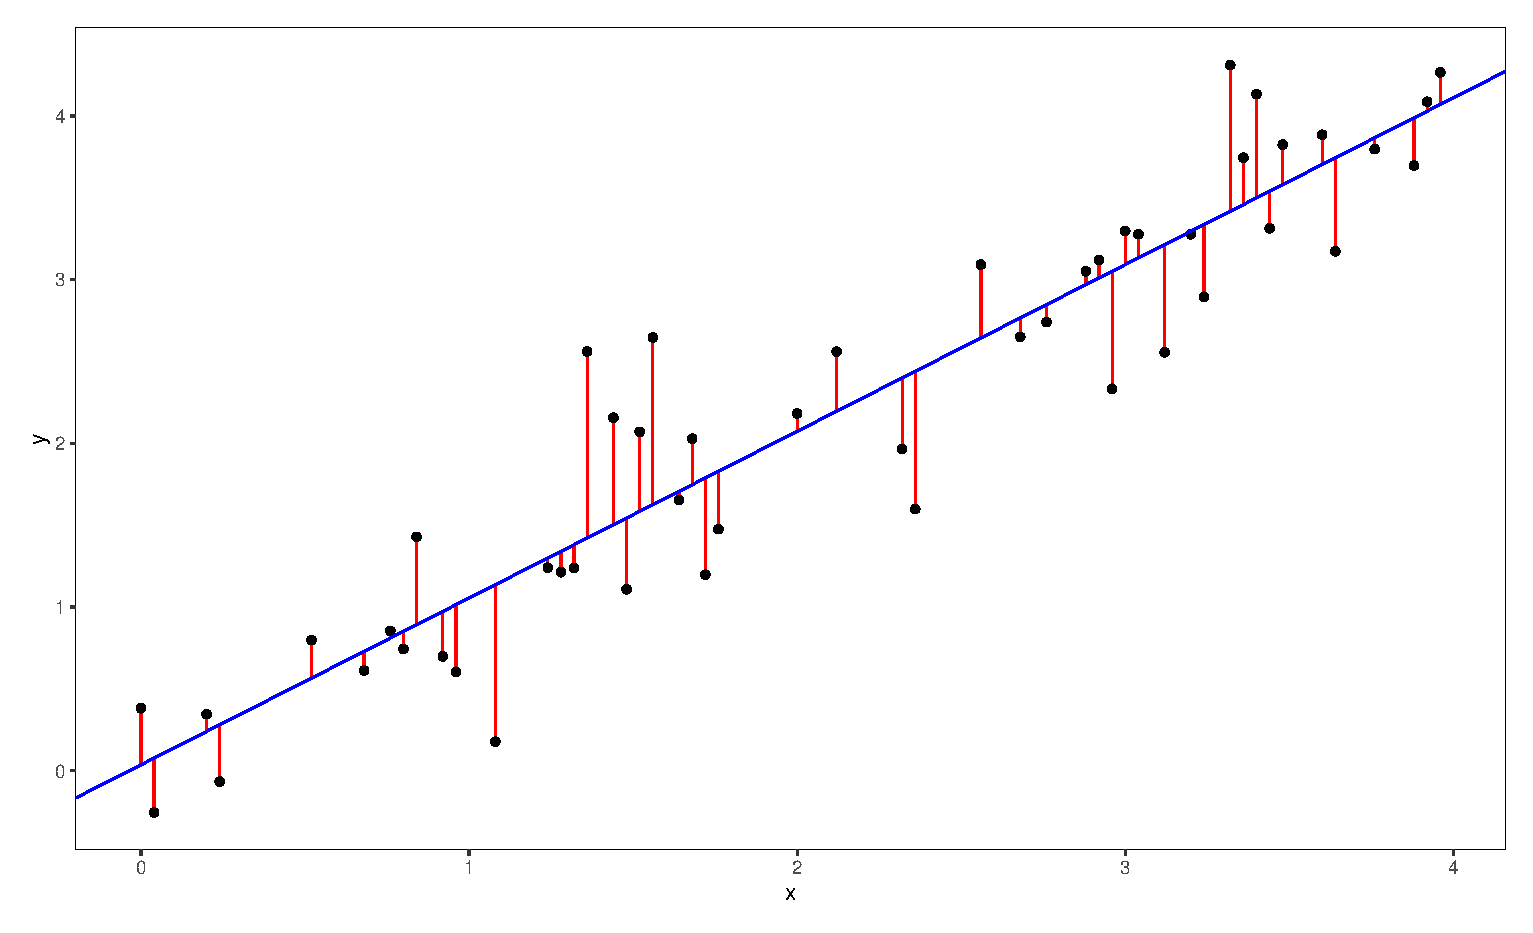
\includegraphics[width = 4in]{images/ols.eps}
	\captionsetup{width=4in}
	\caption{Ordinary least squares fitting with one predictor using simulated data. The blue line represents the line found by ordinary least squares, and the red line segments are the residuals.}
	\label{fig:ols}
\end{figure}

One reason that ordinary least squares is popular is because it is very easy to compute. Let $\beta = [\beta_0, \beta_1, \beta_2, \dotsc, \beta_p]^\top$ be a $(p + 1) \times 1$ vector of coefficient values and let $\mathbf{X}$ be a $n\times (p + 1)$ matrix where each row contains the predictor values for one observation (with an extra value of 1 in the first entry). Then $\mathbf{X}\beta$ is a vector of the estimated response values. Let $\mathbf{y}$ represent the true response values. Then $\mathbf{y} - \mathbf{X}\beta$ is a vector of residuals. To minimize the residual sum of squares, we compute
\begin{equation}
	\hat{\beta}^{\text{OLS}} = \argmin{\beta}{(\mathbf{y} - \mathbf{X}\beta)^\top (\mathbf{y} - \mathbf{X}\beta)}
\end{equation}
where $(\mathbf{y} - \mathbf{X}\beta)^\top (\mathbf{y} - \mathbf{X}\beta)$ is the same residual sum of squares seen in Equation \ref{eqn:RSS}. From \cite{friedman2001elements}, this gives us the solution
\begin{equation}
	\hat{\beta}^{\text{OLS}} = (\mathbf{X}^\top \mathbf{X})^{-1} \mathbf{X}^\top \mathbf{y}
\end{equation}

TODO: Discuss Gauss-Markov Theorem and problems with OLS.

\subsection{Literature Review}
% We can review some relevant literature such as Tibshrani et. al. lasso methods, ridge regression, enet, SCAD, or whatever else we want to do.

Liu et. al. in \cite{liu2020logsum} describe three types of variable selection algorithms: filter methods, which evaluate the ability for each variable to predict the response individually; wrapper methods, which find a subset of predictors highly correlated to the response using feature assessment metrics; and embedded methods, which perform variable selection during the model training process. This paper focuses on the second and third types.

Subset selection methods attempt to find a subset of the predictors that are most correlated with the response variable. Although subset selection techniques can be applied to many types of models, we will focus on subset selection with linear regression.

There are two main benefits to using subset selection methods. By reducing the set of available predictors to just those that are strongly related to the response, overfitting can be mitigated by ignoring unimportant predictors. Another benefit of subset selection is that it creates a more interpretable model, since the fitted model only depends on a few of the predictors.

\textbf{Best subset selection} is a subset selection method that fits considers every possible combination of predictors. For every possible subset size $k$ between 0 and $p$, best subset selection will fit the ${p\choose k}$ possible models using $k$ predictors and chooses the best model. Then, a final model can be selected from the $(p + 1)$ remaining models. The best model is selected using a metric such as the residual sum of squares. Although best subset selection is guaranteed to find the subset of predictors that optimize the chosen metric, this method is computationally expensive. For a data set with $p$ predictors, $2^p$ possible combinations must be considered. This makes best subset selection infeasible when the number of predictors is too large.

Two alternative methods to best subset selection are \textbf{forward selection} and \textbf{backward selection}. Forward selection begins by fitting a model with no predictors and iteratively adds predictors into the model. The predictor added at each step is chosen to best increase the model fit. Conversely, backward selection starts from the full model with all $p$ predictors and repeatedly removes predictors. Then, like best subset selection, the final model is chosen from the candidate models fitted at each step. Although forward and backward selection are not guaranteed to encounter the best possible model, these methods avoid the exponential runtime of best subset selection. Consequently, forward and backward selection can be used for larger values of $p$.

The models produced by forward and backward selection can be improved by allowing for predictors to be added and removed in the same algorithm. \textbf{Forward stepwise selection} begins with a model iteratively improves the model by either adding a new predictor or removing an obsolete one. \textbf{Backward stepwise selection} works in the same way but starts with the full model. These techniques take longer to run than ordinary forward and backward selection, but they are more likely to find the best possible model.

[Discuss AIC/BIC]

\textbf{Ridge regression} helps to solve multicollinearity in predictors while also minimizing insignificant predictors \cite{hoerl1970ridge}. While it does not minimize these insignificant predictors completely to 0 and thus cannot be considered a variable selection method, it still proves very useful in large datasets.

Ridge regression works by minimizing Residual Sum Squared (RSS) plus a penalty as seen in Equation \ref{ridge_reg}. $\lambda$ is a tuning parameter and can be used to determine how much of an effect the penalty has on the regression. if $\lambda=0$, then the regression acts exactly like ordinary least squares regression, but if $\lambda \rightarrow \infty$, then $\beta_j \rightarrow 0$ and the regression line will be a horizontal line at the intercept, $\beta_0$.

\begin{equation}
	\hat{\beta}^{\text{ridge}} = \argmin{\beta}{\sum_{i=1}^{n} \left( y_i - \beta_0 - \sum_{j=1}^{p} \beta_jx_{ij} \right)^2 + \lambda \sum_{j=1}^{p} \beta_j^2  }
	\label{ridge_reg}
\end{equation}

An alternative way to express ridge regression is with the equation
\begin{equation}
	\hat{\beta}^{\text{ridge}} = \argmin{\beta}{\sum_{i=1}^{n} \left( y_i - \beta_0 - \sum_{j=1}^{p} \beta_jx_{ij} \right)^2}\quad\text{subject to}\quad \sum_{j=1}^{p} \beta_j^2\leq t
\end{equation}
for some tuning parameter $t$.

The \textbf{least absolute shrinkage and selection operation}, often referred to as LASSO, is a shrinkage method with a very similar form to lasso regression \cite{tibshirani1996regression, james2017islr, james2013introduction}. The coefficient estimates satisfy
\begin{equation}
	\hat{\beta}^{\text{lasso}}=\argmin{\beta}{\sum\limits_{i = 1}^n \left( y_i - \beta_0 - \sum\limits_{j = 1}^p \beta_j x_{ij} \right) + \lambda\sum\limits_{j = 1}^p \vert \beta_j \vert}
\end{equation}
If $\lambda = 0$, then the lasso model is equivalent to the ordinary least squares model; if $\lambda \to \infty$, then the coefficients for all predictors will be set to 0. An equivalently way to define lasso regression is by
\begin{equation}
	\hat{\beta}^{\text{lasso}} = \argmin{\beta}{\sum_{i=1}^{n} \left( y_i - \beta_0 - \sum_{j=1}^{p} \beta_jx_{ij} \right)^2 }\quad\text{subject to}\quad \sum_{j=1}^{p} \vert \beta_j \vert\leq t
\end{equation}
where $t$ is a tuning parameter.

One useful property of the lasso method is that it can perform variable selection by setting some coefficients to zero. To understand why lasso regression can perform variable selection whereas ride regression cannot, consider Figure \ref{fig:ridge-lasso-diagram} below. This figure demonstrates the case when $p=2$ and $t = 1$. The circle in \ref{fig:ridge-diagram} represents the condition $\beta_1^2 + \beta_2^2 < 1$ for ridge regression, while the red diamond in Figure \ref{fig:lasso-diagram} represents the condition $\vert \beta_1 \vert + \vert \beta_2 \vert < t$ for lasso regression. The blue curves represent contours of the residual sum of squares for values of $\beta_1$ and $\beta_2$. The black point in the center of these curves is where the RSS is minimized; this represents the values of $\beta_1$ and $\beta_2$ that would be selected by ordinary least squares.

\begin{figure}[!h]
	\caption{RSS contours and penalty bounds for the ridge and lasso models when $p=2$ and $t = 1$.}
	\label{fig:ridge-lasso-diagram}
	\centering
	\begin{subfigure}[b]{0.45\textwidth}
		\caption{RSS contours and the ridge penalty boundary.}
		\label{fig:ridge-diagram}
		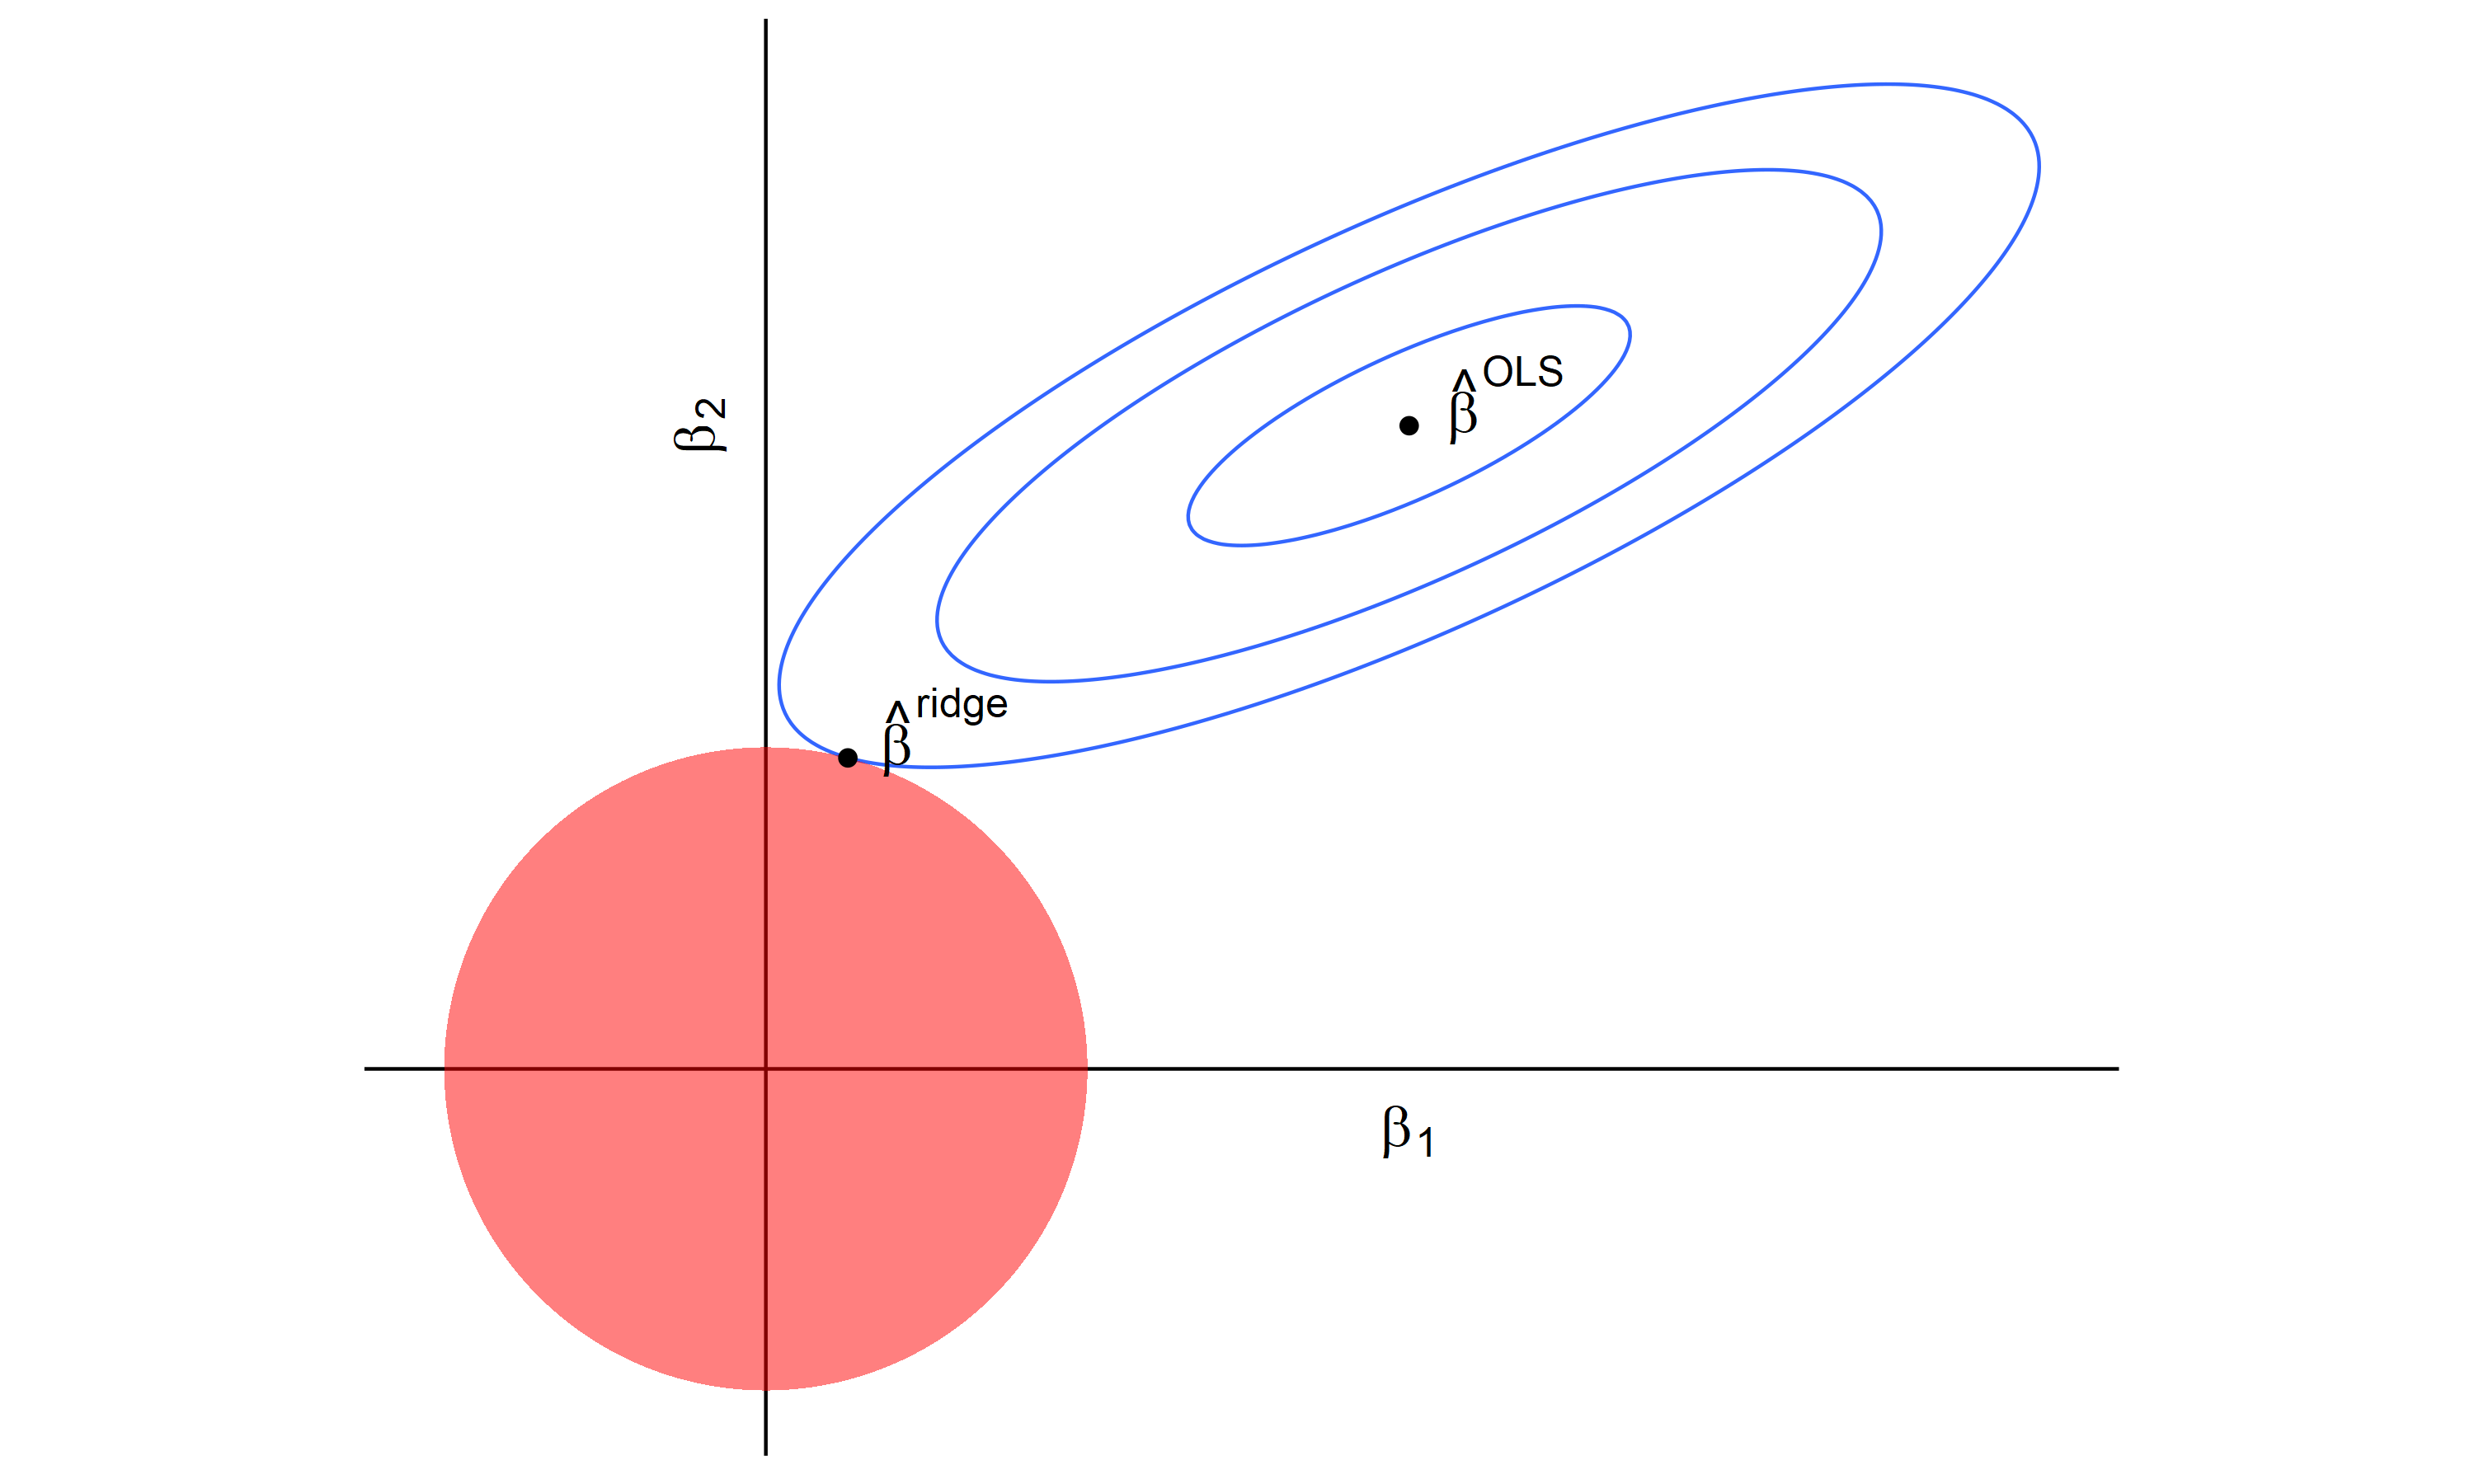
\includegraphics[width=\textwidth]{images/ridge-diagram.png}
	\end{subfigure}
	\hspace{30pt}
	\begin{subfigure}[b]{0.45\textwidth}
		\caption{RSS contours and the lasso penalty boundary.}
		\label{fig:lasso-diagram}
		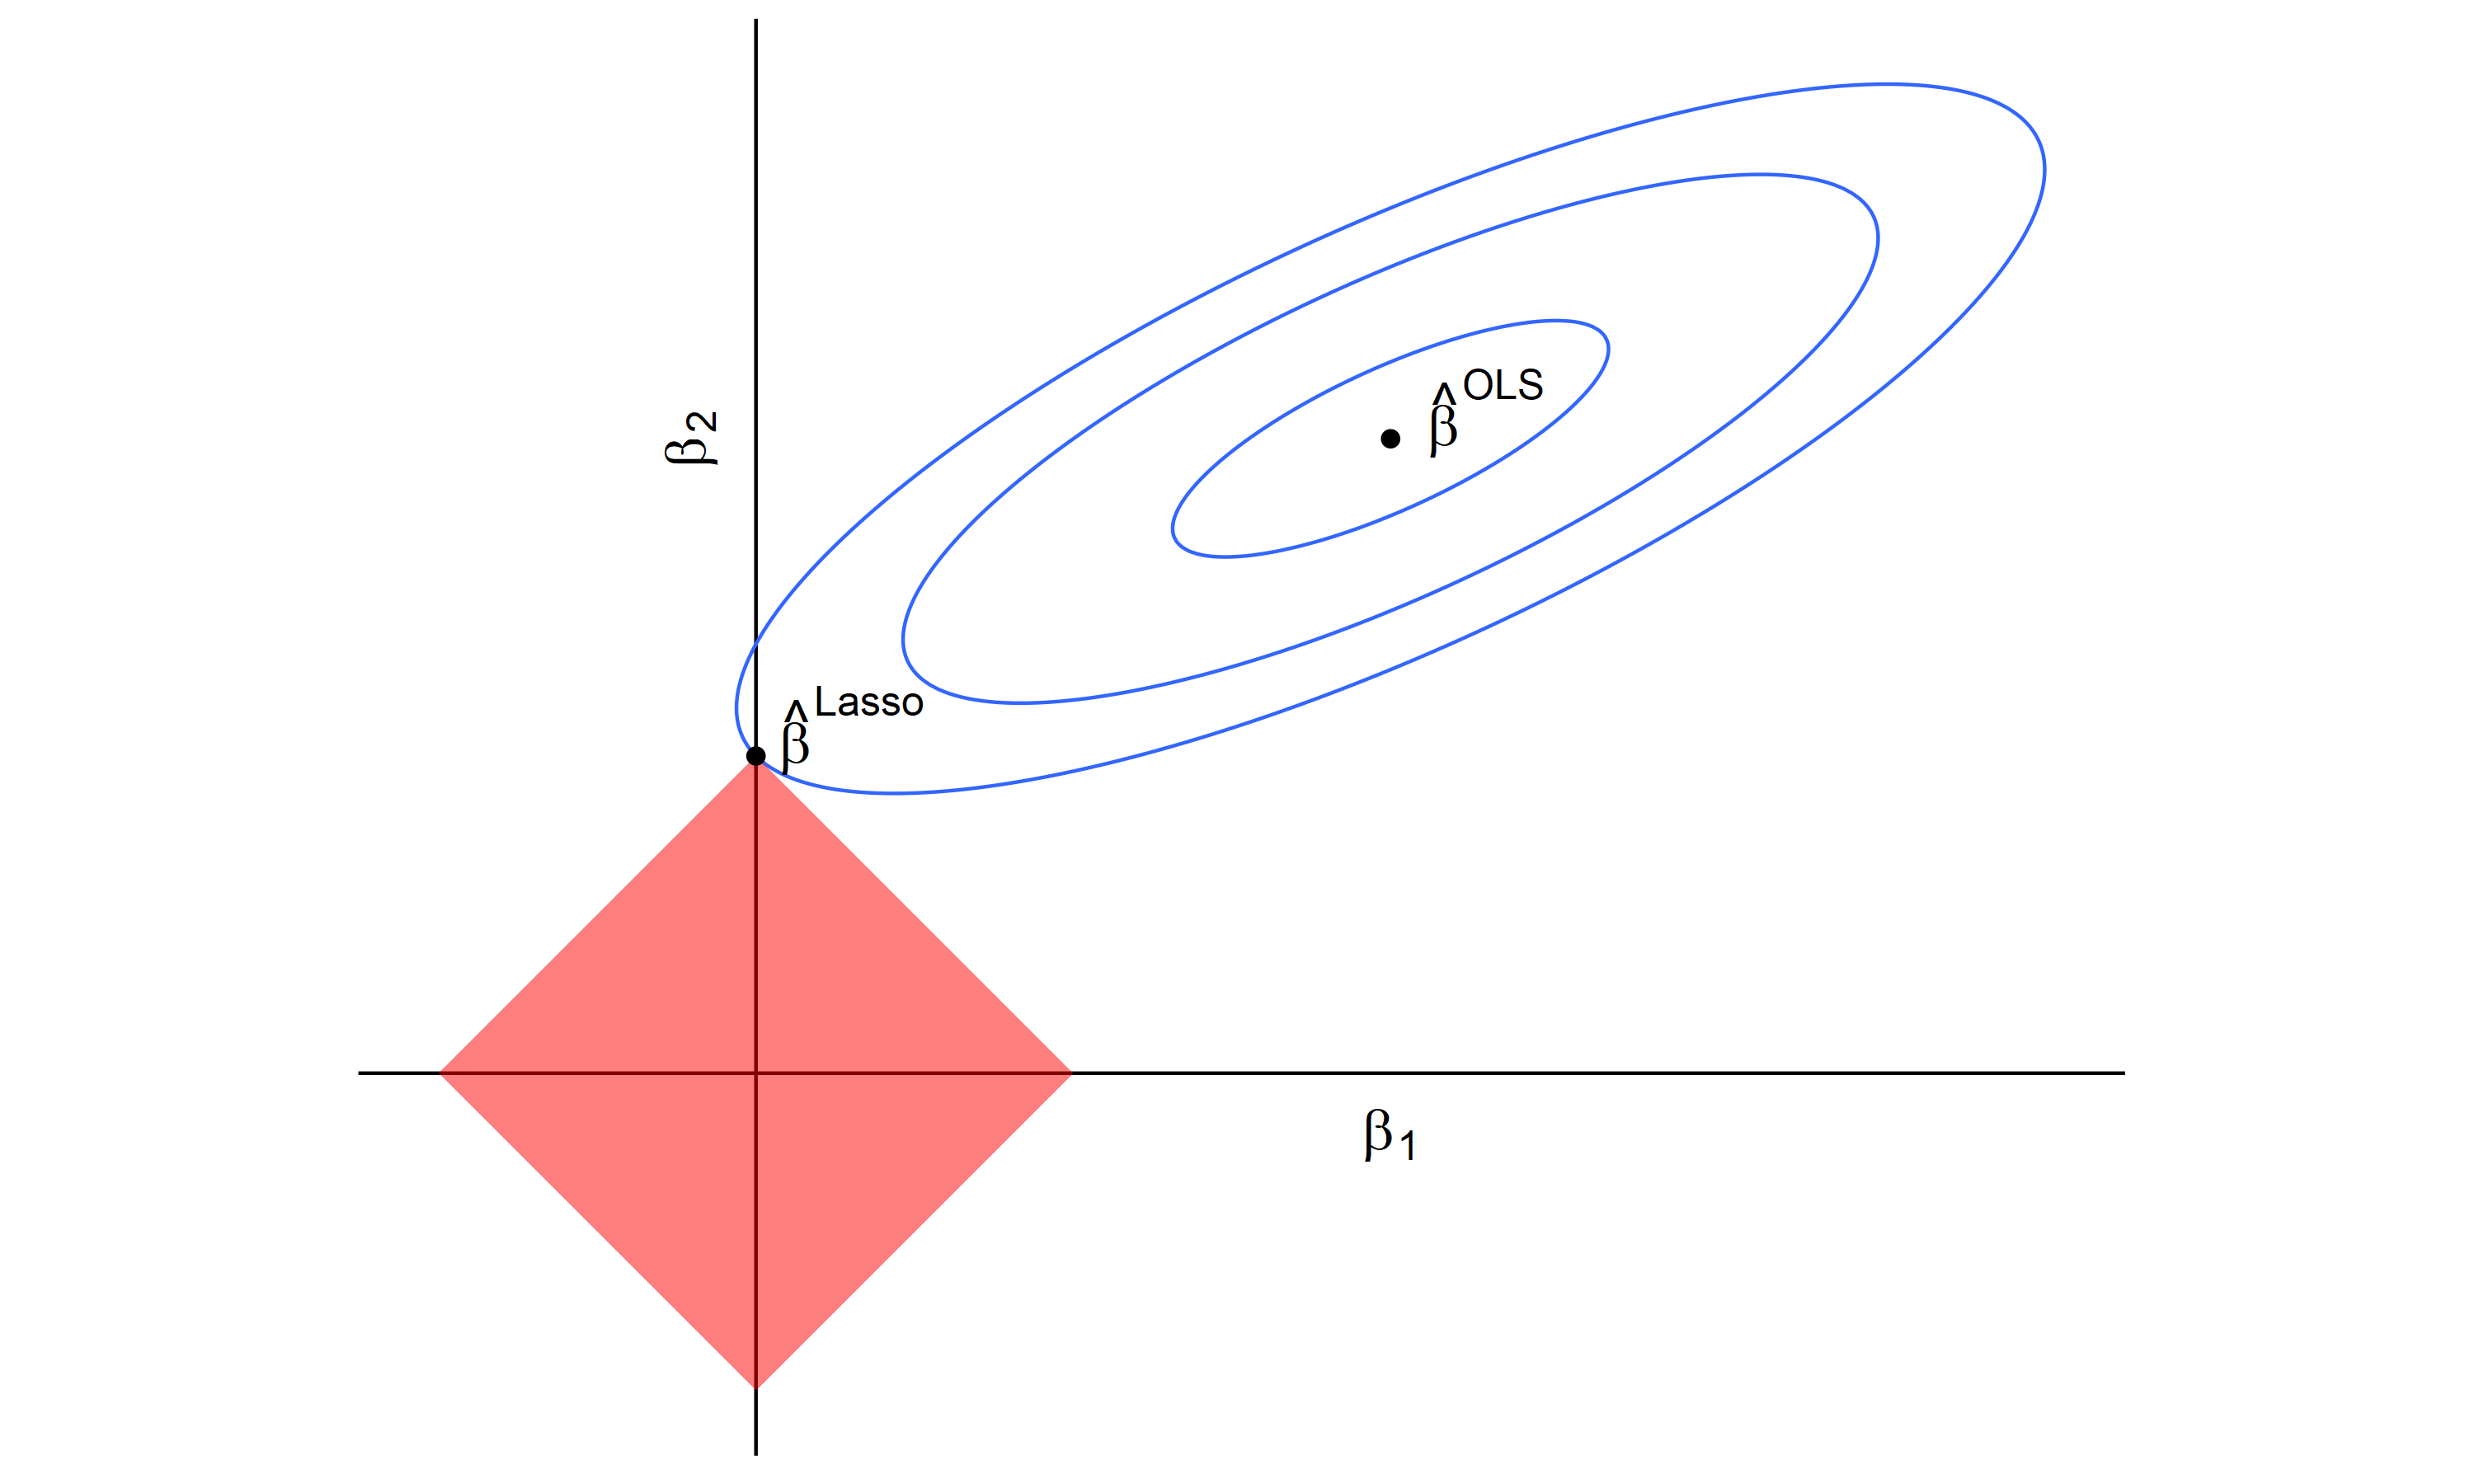
\includegraphics[width=\textwidth]{images/lasso-diagram.png}
	\end{subfigure}
\end{figure}

In \ref{fig:ridge-diagram}, the intersection of the black curve and the red diamond represents the parameter values chosen by ridge regression; this point minimizes the RSS under the condition $\beta_1^2 + \beta_2^2 \leq 1$. Because the red region is a circle, this intersection cannot occur exactly at $\beta_1 = 0$; hence, the ridge method cannot remove the predictor $\beta_1$. On the other hand, the square shape of the constrained region for lasso regression can perform variable selection because the intersection occurs at one of the axes.

The lasso method is particularly useful in the case where $p>n$ because of its ability to select variables; a model with fewer variables has less variance and is more interpretable. One major downside of lasso regression is that it does not handle multicollinearity as nicely as ridge regression. Another downside of lasso regression is that it does not have a closed-form solution, which can lead to instability in the model.

\textbf{Elastic-net} regression serves as a combination between ridge and lasso regression. It can handle  multicollinearity as well as perform variable selection. The coefficients for elastic net regression can be determined by 
\begin{equation}
	\hat{\beta}^{\text{ENet}}=\argmin{\beta}{\sum\limits_{i = 1}^n \left( y_i - \beta_0 - \sum\limits_{i = 1}^p \beta_j x_{ij} \right) + \lambda_2\sum\limits_{j = 1}^p \beta_j^2 + \lambda_1\sum\limits_{j = 1}^p \vert \beta_j \vert}
\end{equation}
where $\lambda_1$ and $\lambda_2$ are both tuning parameters to be determined later.

An important limitation to note is that elastic net performs best when it close to either ridge or lasso regression, meaning that either $\lambda_1 >> \lambda_2$ or vice versa \cite{zou2005regularization}. Additionally, because elastic net requires two tuning parameters, this makes it much more difficult to determine the best combination of tuning parameters to minimize error in the regression. However, this problem has been largely solved through by the LARS-EN algorithm developed by Zou et. al. which efficiently solves for the tuning parameters.
% I will add more here later

Normally in lasso regression, each predictor is weighted the same in the penalty function. \textbf{Adaptive lasso regression} is different in that a weight, $\hat{w}_j$ is multiplied to the penalty function. The coefficients for adaptive lasso regression as designed by Zou et. al. \cite{zou2006adaptive} can be defined by
\begin{equation}
	\hat{\beta}^{\text{adaptive}}=\argmin{\beta}{\sum\limits_{i = 1}^n \left( y_i - \beta_0 - \sum\limits_{i = 1}^p \beta_j x_{ij} \right) + \lambda\sum\limits_{j = 1}^p \hat{w}_j\vert \beta_j \vert}
\end{equation}
where $\lambda$ is a tuning parameter to be determined later and $\hat{w}_j$ is defined as $\frac{1}{\vert\hat{\beta}\vert^{\gamma}}$ with $\gamma$ being a chosen parameter greater than 0.

Because of the weight that is implemented in adaptive lasso regression, zero-coefficients have a weight that is inflated up to infinity, and thus are punished much more harshly than large coefficients whose weight is much smaller in comparison. This is a similar rationale to SCAD and helps to reduce some of the bias from lasso regression. Bridge regression is the general form of lasso regression from which adaptive lasso originates from. When $\gamma < 1$, bridge regression as shown in Equation \ref{adap_lasso} is not continuous, which results in model prediction instability. However, adaptive lasso regression is completely continuous and thus has much more consistent coefficients when fitted.
% I will add more here in the future

\begin{equation}
	\hat{\beta}^{\text{lasso}}=\argmin{\beta}{\sum\limits_{i = 1}^n \left( y_i - \beta_0 - \sum\limits_{i = 1}^p \beta_j x_{ij} \right) + \lambda\sum\limits_{j = 1}^p \vert \beta_j \vert ^\gamma}
	\label{adap_lasso}
\end{equation}


One major flaw of the lasso method is that the penalty punishes large coefficients, even if those coefficients should be large. One way to modify the lasso method is to use the \textbf{smoothly clipped absolute deviation} (SCAD) penalty \cite{fan2001variable}. The goal of this method is to punish large coefficients less severely, which can help mitigate some of the bias introduced by the lasso method.
\begin{equation}
	\hat{\beta}^{\text{SCAD}}=\argmin{\beta}{\sum\limits_{i = 1}^n \left( y_i - \beta_0 - \sum\limits_{i = 1}^p \beta_j x_{ij} \right) + \lambda\sum\limits_{j = 1}^p J_a(\beta_j, \lambda)}
\end{equation}
Here, $J_a(\beta, \lambda)$ is a penalty function that satisfies
\begin{equation}
	\frac{dJ_a(\beta, \lambda)}{d\beta} = \lambda\cdot\sign(\beta)\left[ I(\vert \beta \vert<\lambda) + \frac{(a\lambda - \vert \beta\vert)_+}{(a - 1)\lambda}I(\vert \beta \vert > \lambda) \right]
\end{equation}
where $\lambda \geq 0$ and $a\geq 2$ are tuning parameters. An equivalent way to write this is
\begin{equation}
	\frac{dJ_a(\beta, \lambda)}{d\beta}\left\{\begin{array}{ll}
		\lambda,&\vert \beta \vert\leq \lambda\\
		\frac{a\lambda - \vert \beta \vert}{a - 1},&\lambda < \vert \beta \vert < a\lambda\\
		0,&\alpha\lambda < \vert \beta \vert
	\end{array}\right.
\end{equation}
This penalty function does not punish coefficients with large magnitude as heavily as the lasso method. In fact, if the magnitude of a coefficient is larger than $a\lambda$, then the penalty becomes constant. See Figure \ref{fig:penalty} for a plot of the SCAD penalty as a function of the coefficient value.

Integrating with respect to $\beta$ \cite{breheny2016lasso}, we see that
\begin{equation}
	J_a(\beta, \lambda) = \left\{\begin{array}{ll}
		\lambda \vert \beta \vert,&\vert \beta \vert \leq \lambda\\
		\frac{2a\lambda\vert\beta\vert - \beta^2-\lambda^2}{2(a - 1)},&\lambda < \vert \beta \vert < a\lambda\\
		\frac{\lambda^2(a + 1)}{2},&a\lambda < \vert \beta \vert
	\end{array}\right.
\end{equation}

The \textbf{minimax concave penalty} (MCP) method is very similar to smoothly clipped absolute deviation \cite{zhang2010nearly, breheny2016lasso}. Both methods are used to avoid the high bias caused by the lasso method. MCP uses a penalty function that satisfies
\begin{equation}
	\frac{dJ_a(\beta, \lambda)}{d\beta} = \left\{\begin{array}{ll}
		\sign(\beta)\left(\lambda - \frac{\vert \beta \vert}{a}\right),& \vert \beta \vert \leq a\lambda\\
		0,&a\lambda < \vert \beta \vert
	\end{array}\right.
\end{equation}
where $\lambda\geq 0$ and $a> 0$ are tuning parameters. Integrating \cite{breheny2016lasso}, we see that
\begin{equation}
	J_a(\beta, \lambda) = \left\{\begin{array}{ll}
		\lambda \vert \beta \vert - \frac{\beta^2}{2a},&\vert \beta \vert \leq a\lambda\\
		\frac{1}{2}a\lambda^2,&a\lambda < \vert \beta \vert
	\end{array}\right.
\end{equation}

Figure \ref{fig:lasso-scad-mcp} below shows the penalty functions (and their derivatives) for LASSO, SCAD, and MCP as a function of a coefficient value $\beta$. We see that LASSO applies a much stronger penalty to large coefficients than SCAD or MCP. Also, note that SCAD starts with a derivative equal to that of the lasso for small values of $\beta$; on the other hand, the derivative of the penalty function for MCP starts decreasing immediately.

\begin{figure}[!h]
	\caption{Penalty functions for LASSO, SCAD, and MCP, as well as their derivatives. These plots use $\lambda = 2$ and $a = 3$.}
	\label{fig:lasso-scad-mcp}
	\centering
	\begin{subfigure}[b]{0.4\textwidth}
		\caption{Penalty functions for LASSO, SCAD, and MCP}
		\label{fig:penalty}
		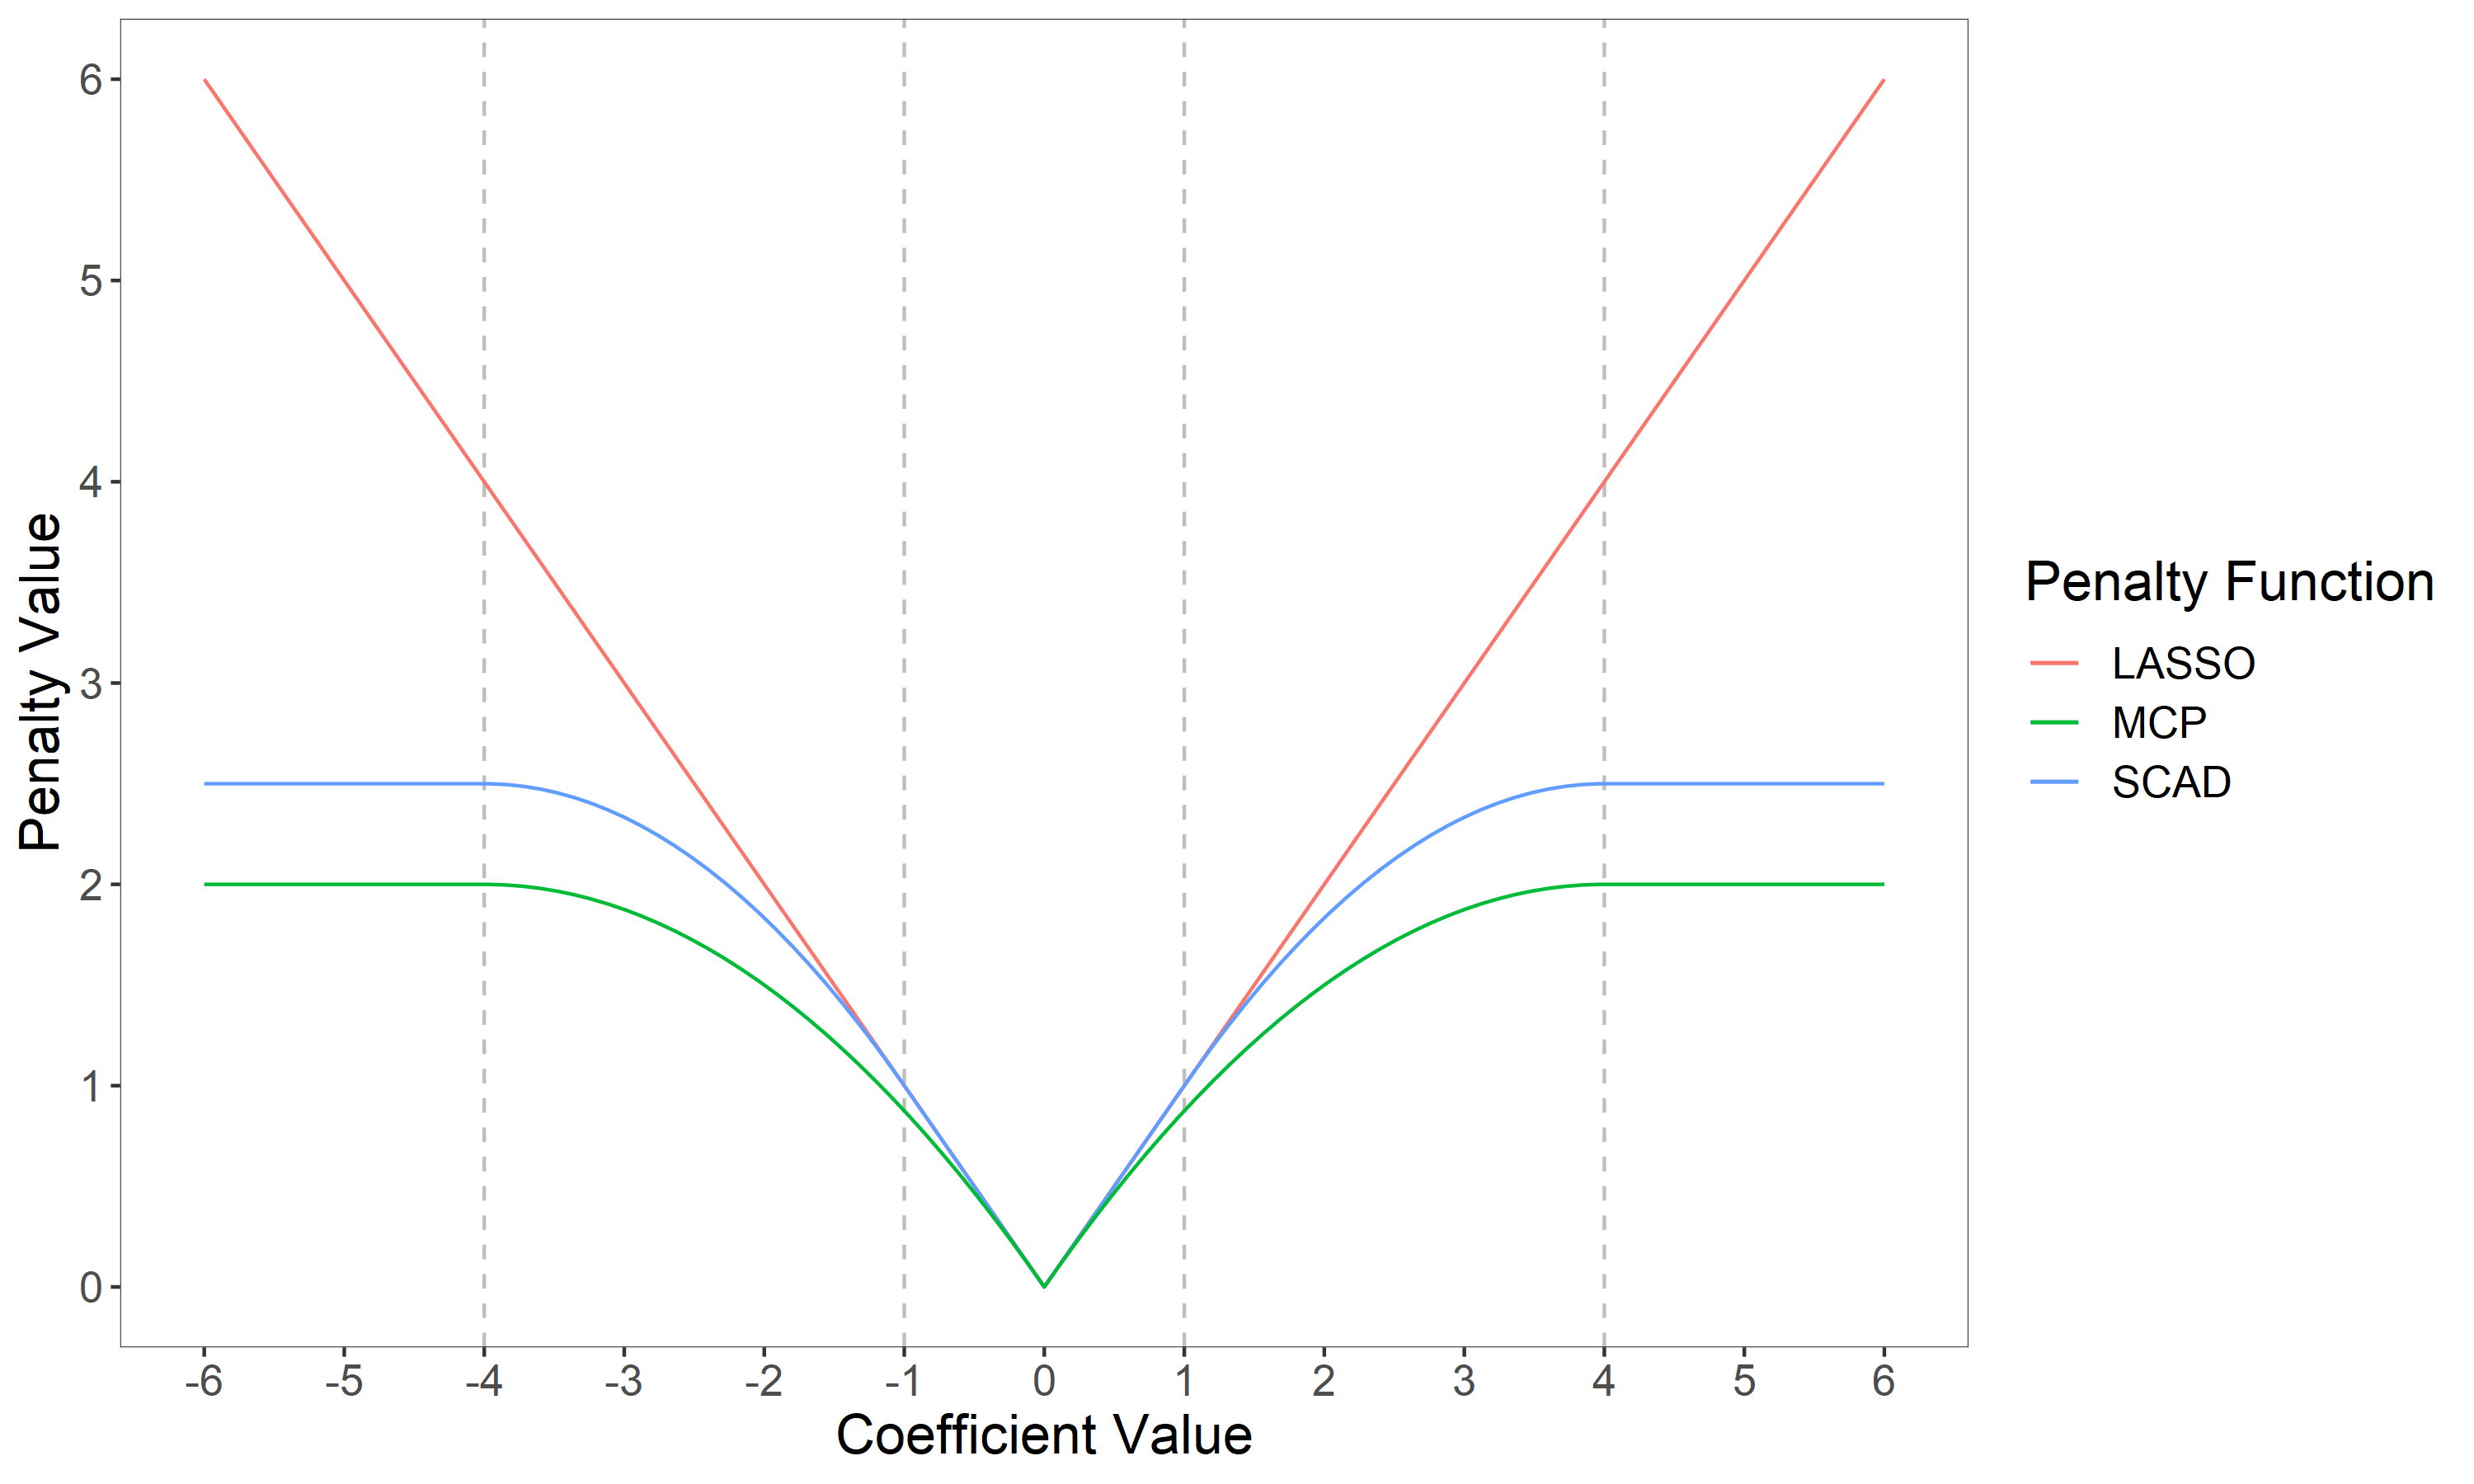
\includegraphics[width=\textwidth]{images/lasso-scad-mcp-penalty.png}
	\end{subfigure}
	\hspace{30pt}
	\begin{subfigure}[b]{0.4\textwidth}
		\caption{Derivatives of the penalty functions for LASSO, SCAD, and MCP}
		\label{fig:derivative}
		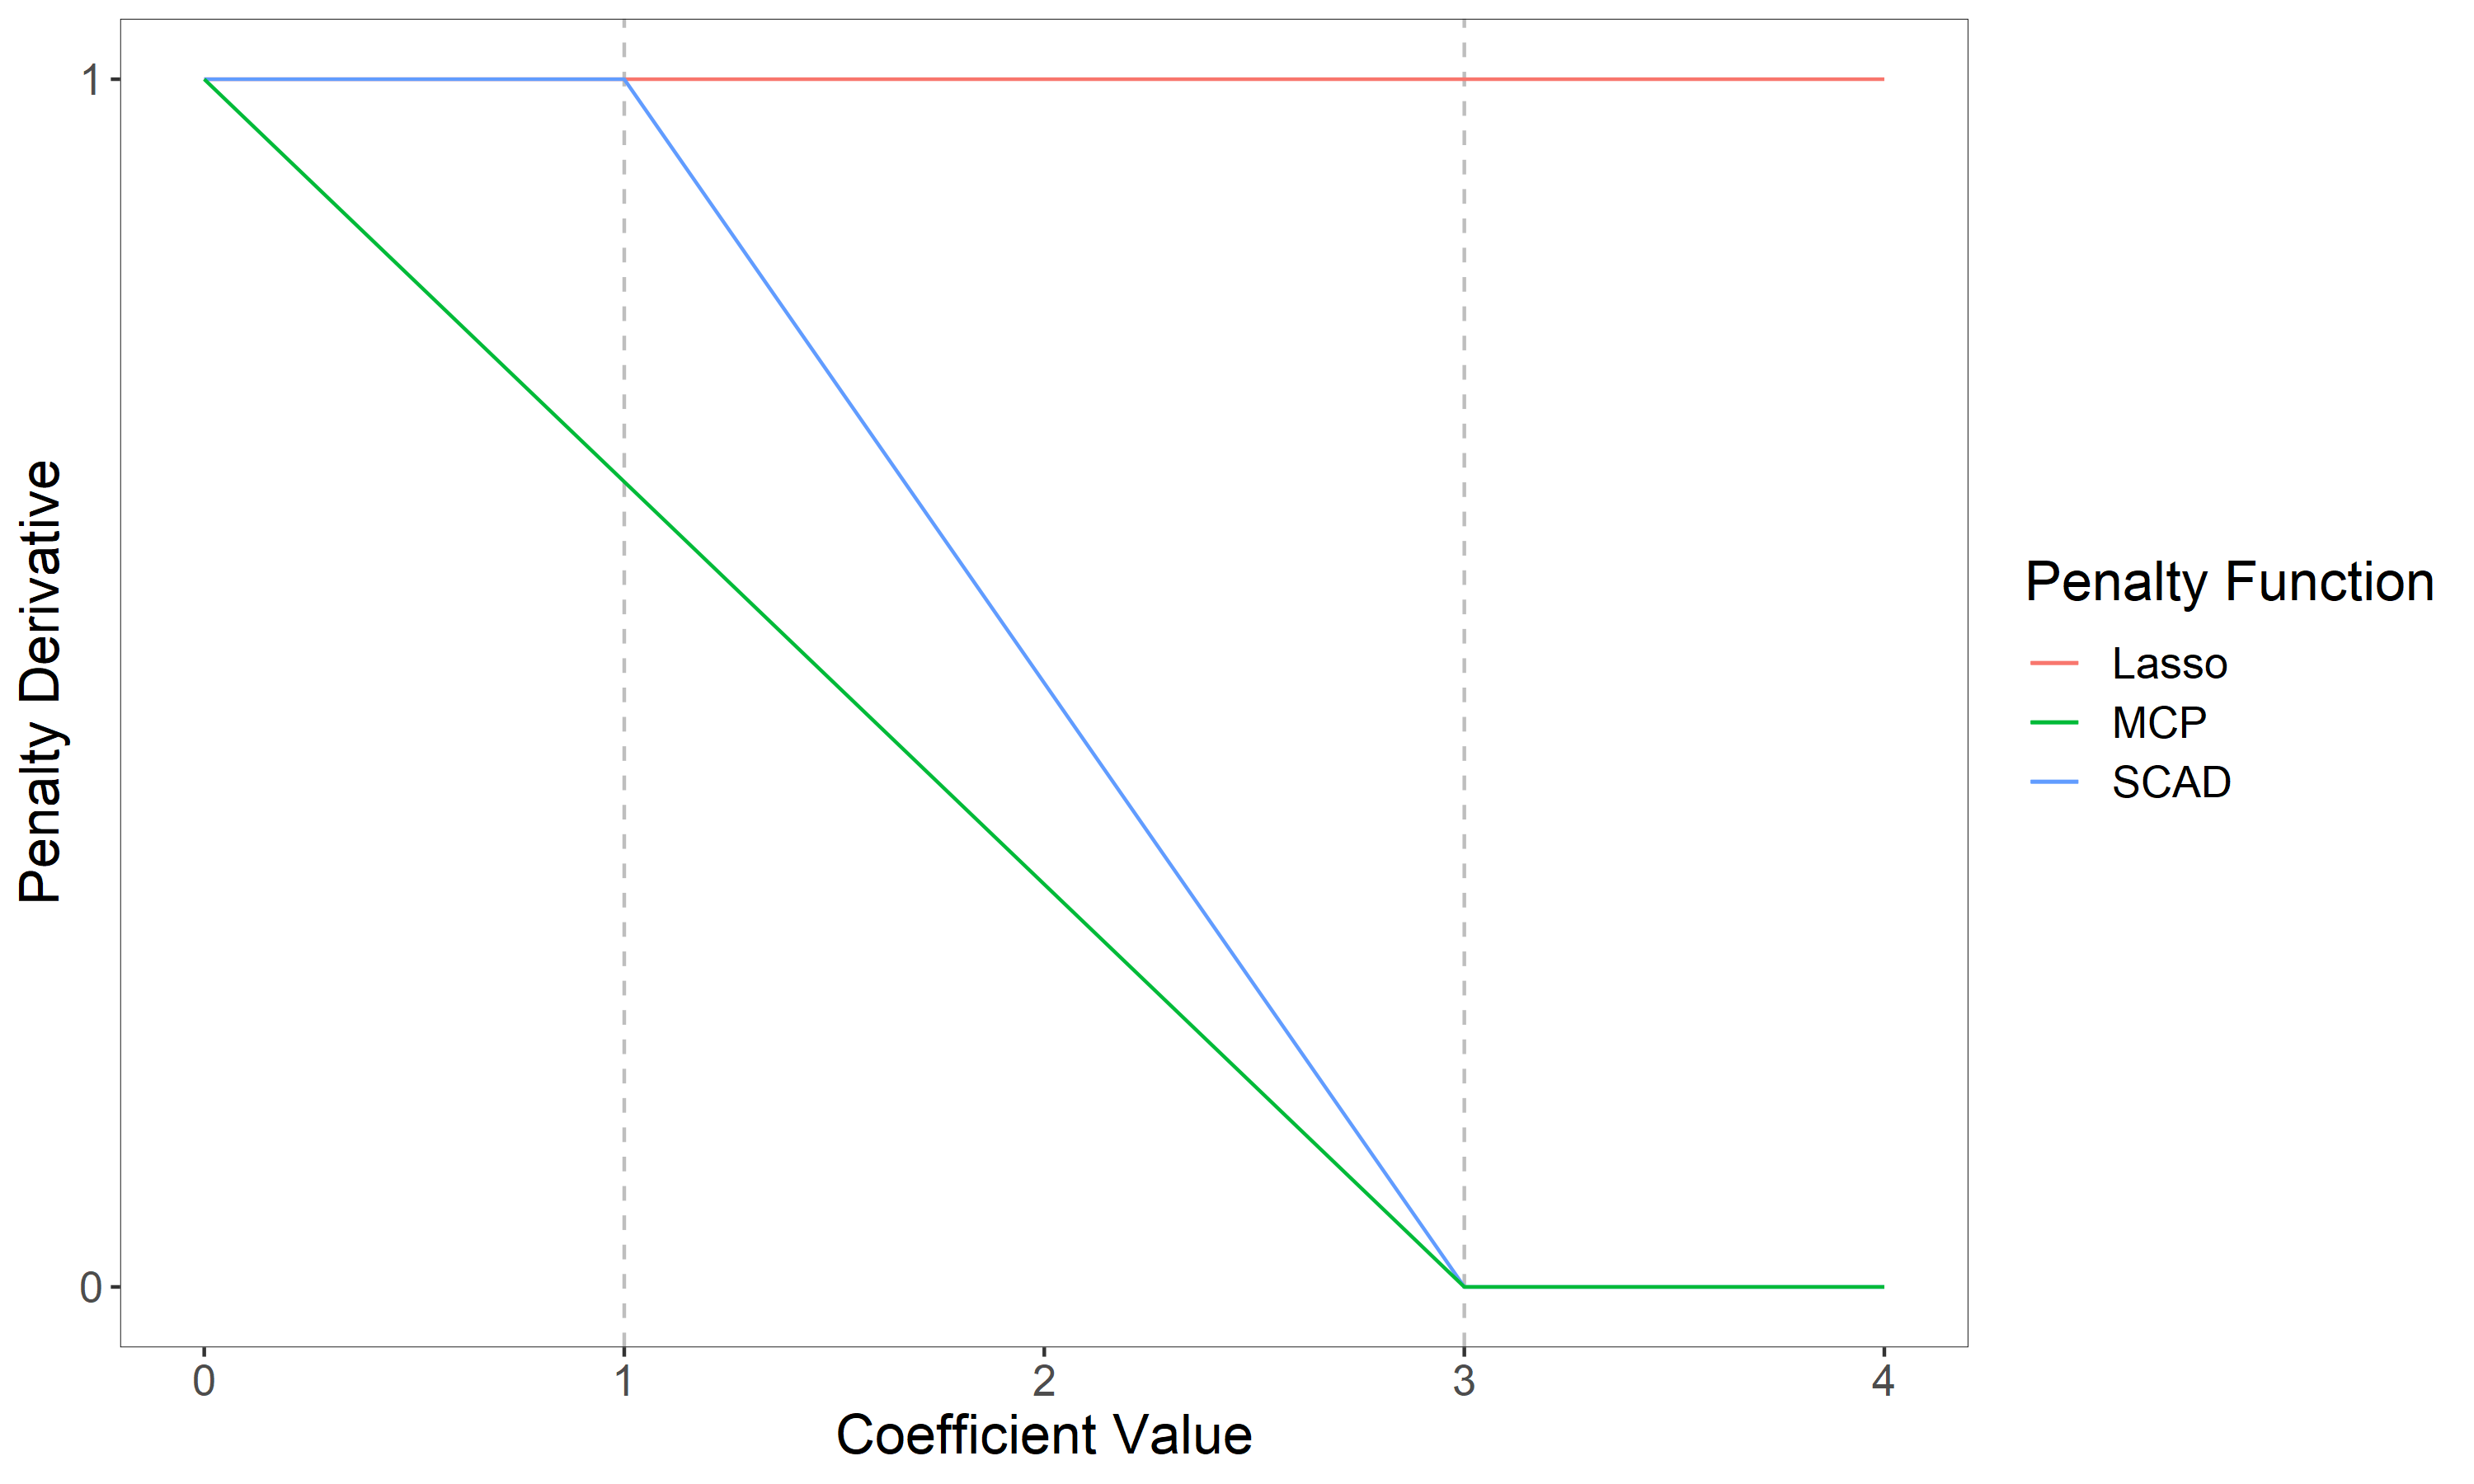
\includegraphics[width=\textwidth]{images/lasso-scad-mcp-derivative.png}
	\end{subfigure}
\end{figure}

Now, consider the case where $p=1$ (there is only one predictor). Figure \ref{fig:prediction} shows the solutions given when using LASSO, SCAD, and MCP on such a model. The $x$-axis gives the actual coefficient for the single variable, and the $y$-axis represents the coefficient estimate produced using each of the algorithms. We used the particular values $\lambda = 2$ and $a = 3$. The gray line is the identity function, which also equals the solution obtained using ordinary least squares.

We see that all three methods set the predicted value to zero when the actual coefficient is small. Also, note that the LASSO method is always off from the identity function when the coefficient is large. On the other hand, SCAD and MCP merge with the identity function when the coefficient is sufficiently large. This shows that both SCAD and MCP can avoid the high bias that LASSO introduces.

\begin{figure}[!h]
	\centering
	\caption{Solutions for LASSO, SCAD, and MCP for a single predictor when $\lambda=2$, and $a = 3$.}
	\label{fig:prediction}
	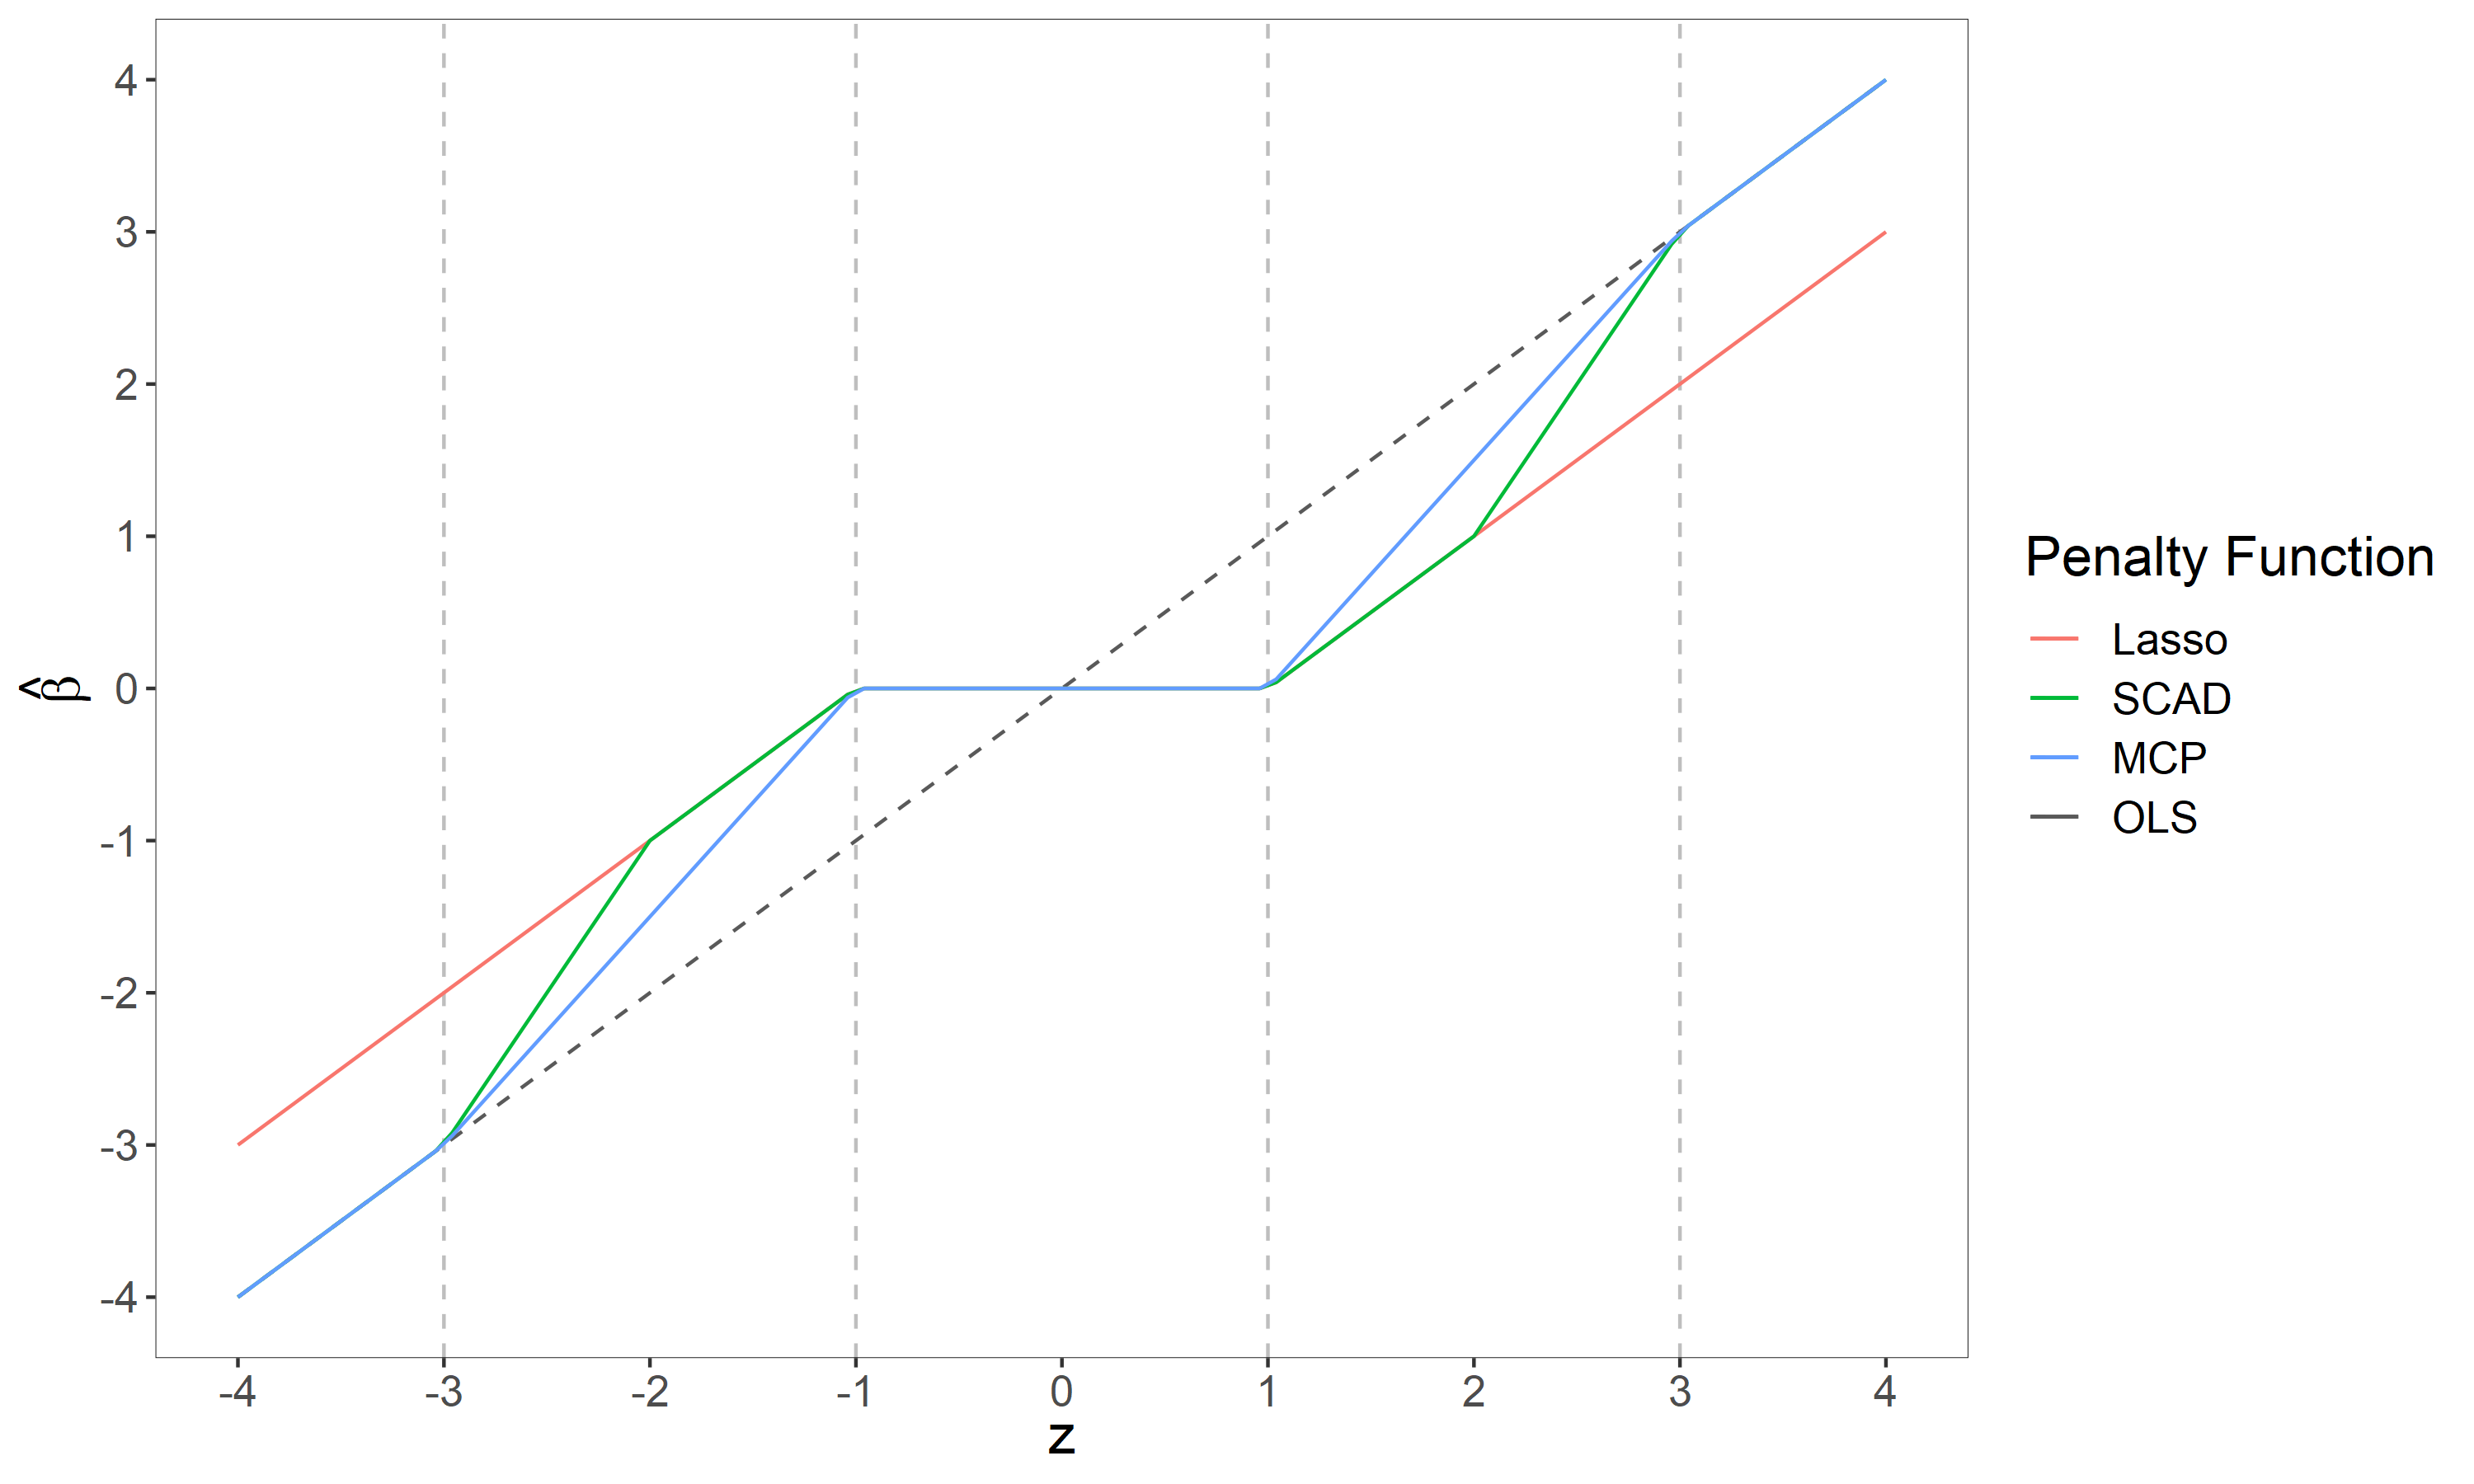
\includegraphics[width = 0.4\textwidth]{images/lasso-scad-mcp-solution.png}
\end{figure}

%%%%%%%%%%%%%%%%%%%%%%%%%%%%%%%%%%%%%%%%%%%%%%%%%%%%%%%%%%%%%%%%%%%%%
\section{Methods}
\subsection{Models}
% lists and describes every tested model. Can include equations for models, but should not go into such great depth about each model: that can be reserved for literature review portion of the paper.

\subsection{Monte Carlo Simulations}
% outline data generation process and factorial design process

Monte Carlo simulations use randomly generated data to fit and test our regression and classification models. There are several benefits to using simulated data rather than experimental data:
\begin{itemize}
	\item The true relationship between the predictor variables and the response is known.
	\item Simulations can be iterated many times, giving sturdier results about the effectiveness of each model.
	\item We have full control over factors such as the number of predictors and the amount of correlation between predictors.
\end{itemize}

For the simulated data, we assumed that the relationship between the response variable $y$ and the predictors $x_1, x_2, \dotsc, x_p$ was linear. That is, we assumed that
\begin{equation}
	y = \beta_0 + \beta_1 x_1 + \cdots + \beta_p x_p + \epsilon
\end{equation}
where $\beta_0$ is some intercept, $\beta_1, \dotsc, \beta_p$ are coefficient values and $\epsilon\sim \mathcal{N}(0, \sigma^2)$ is a normally distributed random error with mean 0 and variance $\sigma^2$.

To generate the data, we first defined $\beta = [\beta_0, \beta_1, \dotsc, \beta_p]^\top$, a $(p + 1)\times 1$ vector of coefficient values. For our simulations, we used $\beta_0 = 1$, $\beta_1 = 2$, $\beta_2 = -2$, $\beta_5=0.5$ and $\beta_6 = 3$; the remaining coefficient values were set to 0.

Next, we generated $\mathbf{X}$, a $n\times (p + 1)$ matrix of predictor variables. The first column contains 1 in all of its entries; this corresponds to the intercept of our linear model. Column $i$ of $\mathbf{X}$ contains the variable values for predictor $x_{i - 1}$, for $1\leq i\leq p$. These values were generated using the $p$-dimensional multivariate normal distribution $\mathcal{N}_p(0, \mathbf{\Sigma})$ with mean zero and covariance matrix $\mathbf{\Sigma}$. We assumed that every predictor had a standard deviation of 1, making the covariance matrix equivalent to a correlation matrix. Four different correlation matrix structures were considered in our study.

We then generated an $n\times 1$ error vector $\mathbf{e}\sim \mathcal{N}(0, \sigma^2)$ with mean zero and variance $\sigma^2$. For regression models, the response $\mathbf{y}$ can then be computed by
\begin{equation}
	\mathbf{y} = \mathbf{X}\beta + \mathbf{e}
\end{equation}

We used a \textbf{factorial design} for our simulations. This means that we considered several factors that affect the data generation process, each having multiple possible values. We then generated data using every possible combination of factor values, giving us a comprehensive assessment of model performance under various conditions.
\begin{itemize}
	\item $n$, the number of observations: 50, 200, 1000.
	\item $p$, the number of predictors: 10, 100, 2000.
	\item $\sigma$, the standard deviation of the random error: 1, 3, 6.
	\item The correlation matrix structure: independent, symmetric compound, autoregressive, blockwise.
	\item $\rho$, the correlation between predictors: 0.2, 0.5, 0.9.
\end{itemize}

By taking every possible combination of these factors, we obtain $3\times 3\times 3\times 4\times 3 = 324$ different settings for the simulations. However, because an independent correlation matrix does not use the correlation value $\rho$, we actually only used 270 combinations. For each combination of factors, we ran 100 simulations. In each simulation, we generated two data sets: one to train the various models, and one to test the models and evaluate performance. Both data sets contained $n$ observations, meaning that a total of $2n$ observations were generated for each simulation.

As mentioned earlier, we considered four different covariance matrix structures. These structures determine the correlation between different predictors. If $\Sigma$ is a correlation matrix, then $\mathbf{\Sigma_{ij}}$, the entry at the $i$-th row and $j$-th column, represents the correlation between predictors $i$ and $j$. If $\mathbf{\Sigma_{ij}}=0$, there is no correlation; but if $\mathbf{\Sigma_{ij}}=1$, then predictors $i$ and $j$ are perfectly correlated. Note that a correlation matrix is always symmetric, so $\mathbf{\Sigma}_{ij} = \mathbf{\Sigma}_{ji}$ for all indices $i$ and $j$. This correlation can severely impact the performance of statistical models; if several predictors are highly correlated, then machine learning algorithms are less able to determine which predictors are actually related to the response.

The first correlation structure we considered is \textbf{independent correlation}. This means that the correlation matrix $\mathbf{\Sigma}$ has the form
\begin{equation}
	\mathbf{\Sigma} = \begin{bmatrix}
		1 & 0 & \cdots & 0 \\
		0 & 1 & \cdots & 0 \\
		\vdots & \vdots & \ddots & \vdots \\
		0 & 0 & \cdots & 1
	\end{bmatrix}
\end{equation}
In other words, there is no correlation between different predictors, since $\mathbf{\Sigma}_{ij} = 0$ whenever $i\neq j$.

The next covariance structure is called \textbf{symmetric compound}. This structure has the form
\begin{equation}\label{eqn:symmetric-compound-matrix}
	\mathbf{\Sigma} = \begin{bmatrix}
		1 & \rho & \cdots & \rho \\
		\rho & 1 & \cdots & \rho \\
		\vdots & \vdots & \ddots & \vdots \\
		\rho & \rho & \cdots & 1
	\end{bmatrix}
\end{equation}
where $\rho \in [0, 1]$ is some correlation value. A symmetric compound covariance structure assumes that $\mathbf{\Sigma}_{ij} = \rho$ whenever $i \neq j$, meaning that all predictors are equally correlated with one another.

An autoregressive covariance structure assumes that
\begin{equation}
	\mathbf{\Sigma} = \begin{bmatrix}
		1 & \rho & \cdots & \rho^{p - 1} \\
		\rho & 1 & \cdots & \rho^{p - 2} \\
		\vdots & \vdots & \ddots & \vdots \\
		\rho^{p - 1} & \rho^{p - 2} & \cdots & 1
	\end{bmatrix}
\end{equation}
For any indices $i$ and $j$, we have $\mathbf{\Sigma}_{ij} = \rho^{\vert i - j\vert}$. Consequently, each predictor is strongly correlated with nearby predictors and weakly correlated with more distant predictors. This form of covariance is commonly seen when using time series, since observed values at nearby times are likely to be highly correlated with one another.

Finally, a blockwise correlation matrix has the block-diagonal form
\begin{equation}
	\mathbf{\Sigma} = \begin{bmatrix}
		\mathbf{B}_1 & 0 & \cdots & 0 \\
		0 & \mathbf{B}_2 & \cdots & 0 \\
		\vdots & \vdots & \ddots & \vdots \\
		0 & 0 & \cdots & \mathbf{B}_k
	\end{bmatrix}
\end{equation}
where $0$ represents a block containing all zeroes, and each block $\mathbf{B}_i$ has a form identical to the symmetric compound matrix in Equation \ref{eqn:symmetric-compound-matrix}. This implies that predictors within the same block have correlation $\rho\in [0, 1]$, whereas predictors in different blocks have zero correlation. One important consideration when using blockwise correlation is the size of each block. For our simulations, we used a block size of 5 when $p = 10$, a block size of 25 when $p = 100$, and a block size of 100 when $p = 2000$.

All of our simulations were run using version 4.1.0 of \lstinline!R!. Several different libraries were used to fit machine learning models using our simulated data. Table \ref{tab:model-libraries} summarizes the libraries used to fit models.

\begin{table}[h]
	\centering
	\caption{\lstinline!R! Libraries used and the models used from each library}
	\label{tab:model-libraries}
	\begin{tabular}{lll}
		\textbf{Library}    & \textbf{Models used}                                 & \textbf{Version} \\ \hline
		\lstinline!stats!   & Ordinary least squares                               & 4.1.0            \\
		\lstinline!MASS!    & Stepwise selection                                   & 7.3-54           \\
		\lstinline!glmnet!  & Ridge, lasso, elastic-net                            & 4.1-1            \\
		\lstinline!gcdnet!  & Adaptive ridge, adaptive lasso, adaptive elastic-net & 1.0.5            \\
		\lstinline!ncvreg!  & SCAD and MCP                                         & 3.13.0           \\
		\lstinline!xgboost! & Gradient boosting                                    & 1.4.1.1          \\
		\lstinline!ranger!  & Random forest                                        & 0.12.1           \\
		\lstinline!e1071!   & Support vector machine                               & 1.7-7           
	\end{tabular}
\end{table}

For ridge, lasso, and elastic-net regression using \lstinline!glmnet!, we used the \lstinline!cv.glmnet! function. This function uses cross-validation to determine the value of $\lambda$ that minimizes the cross-validation error. We used ten folds with \lstinline!cv.glmnet!. Using cross-validation can help generate a model that has a good test performance. For elastic-net regression, we used the hyperparameter $\alpha = 0.8$. This means that the elastic-net model is more similar to lasso (where $\alpha = 1$) than ridge (where $\alpha = 0$). The remaining hyperparameters were given their default values.

We used the \lstinline!cv.gcdnet! function from the \lstinline!gcdnet! library for the adaptive versions of ridge, lasso, and elastic-net. Again, ten folds were used for the cross-validation, and all hyperparameters were given their default values.

For SCAD and MCP models, we used the \lstinline!cv.ncvreg! function from the \lstinline!ncvreg! library. We used the default values of $a$ for both models: 3 for MCP and 3.7 for SCAD (note that the \lstinline!ncvreg! documentation calls this hyperparameter $\gamma$ instead of $a$).

For the three non-linear models (gradient boosting, random forests, and support vector machines), we used cross-validation and grid search to find suitable hyperparameters, and then fit a model using the full training set using those hyperparameters. For gradient boosting with \lstinline!xgboost!, we used different values for the learning rate (0.1, 0.3, and 0.5) and maximum tree depth (1, 3, and 7). A maximum of 1000 trees were generated, with an early stopping condition if the model failed to improve for several iterations in a row. The cross-validation function used five folds.

For random forests using \lstinline!ranger!, we tuned the number of predictors used per decision tree ($\lfloor \sqrt{p}\rfloor$, $\lfloor p / 3 \rfloor$, and $\lfloor p / 2 \rfloor$) and the number of trees (300, 400, 500 and 600). The cross-validation function used five folds.

Finally, for support vector machines using \lstinline!e1071!, we varied $\epsilon$ (TODO: explain this) and the cost function (0.5, 1, and 2).




\subsection{Empirical Data}
% outline empirical data sources and what each database is about / what we try to predict about it

%%%%%%%%%%%%%%%%%%%%%%%%%%%%%%%%%%%%%%%%%%%%%%%%%%%%%%%%%%%%%%%%%%%%%
\section{Results}
\subsection{Regression Models}
% Stick all the results from the linear regression models here

\subsection{Classification Models}
% stick the results from logisitc regression and classification models here

%%%%%%%%%%%%%%%%%%%%%%%%%%%%%%%%%%%%%%%%%%%%%%%%%%%%%%%%%%%%%%%%%%%%%
\section{Discussion}
% discussion of findings, future work, and contributions
\subsection{Findings}
% overall ideas that we found out after all these results. Which type of model is best in which environment, etc?
% Might need to break it into sub sub sections for classification vs regression or monte carlo vs empirical???
\subsection{Contributions}
% what are our contributions, why is what we did important?
% we have a comprehensive analysis of 21 models in 270 different environments. Allows for comprehensive comparison and gives guidance to data scientists as to which model they should use for their research
% empirical data methods show the important uses of penalized regression in environmental, biological, and etc. data
\subsection{Future Work}
% maybe talk about the penalty method we came up with? Talk about how it might be able to solve issues of Logsum method?


\newpage
\bibliographystyle{plain}
\bibliography{references}
\end{document}